Deep learning has been remarkably successful in many areas~\cite{Girshick2014, Krizhevsky2012, Ren2017, Shelhamer2017}. However, many studies find out deep learning methods are hard to generalize when they encounter an unseen domain, which has a different data distribution than domains used for training~\cite{Li2018MLDG, Li2017dg, Li2018MLDG, shankar2018generalizing, ganin2015unsupervised, bousmalis2016domain, motiian2017CCSA}. This problem called \textit{domain shift}~\cite{Shimodaira2000}. For alleviating the domain shift problem, many studies have been carried out on different assumptions. Domain Adaptation (DA) assumes there are two domains. The first is a fully-labeled source domain, and the other is a sparsely labeled or totally unlabeled target domain. Otherwise, domain generalization (DG) assumes there are some fully-labeled source domains, but the target domain is totally unavailable. DG is a challenge but important research area because generalization to other domains is crucial to make a safe artificial intelligence. Moreover, it is helpful to understand how deep neural networks see the world.

\begin{figure}[t]
	\centering
	\footnotesize
	\begin{tabular}{c}
		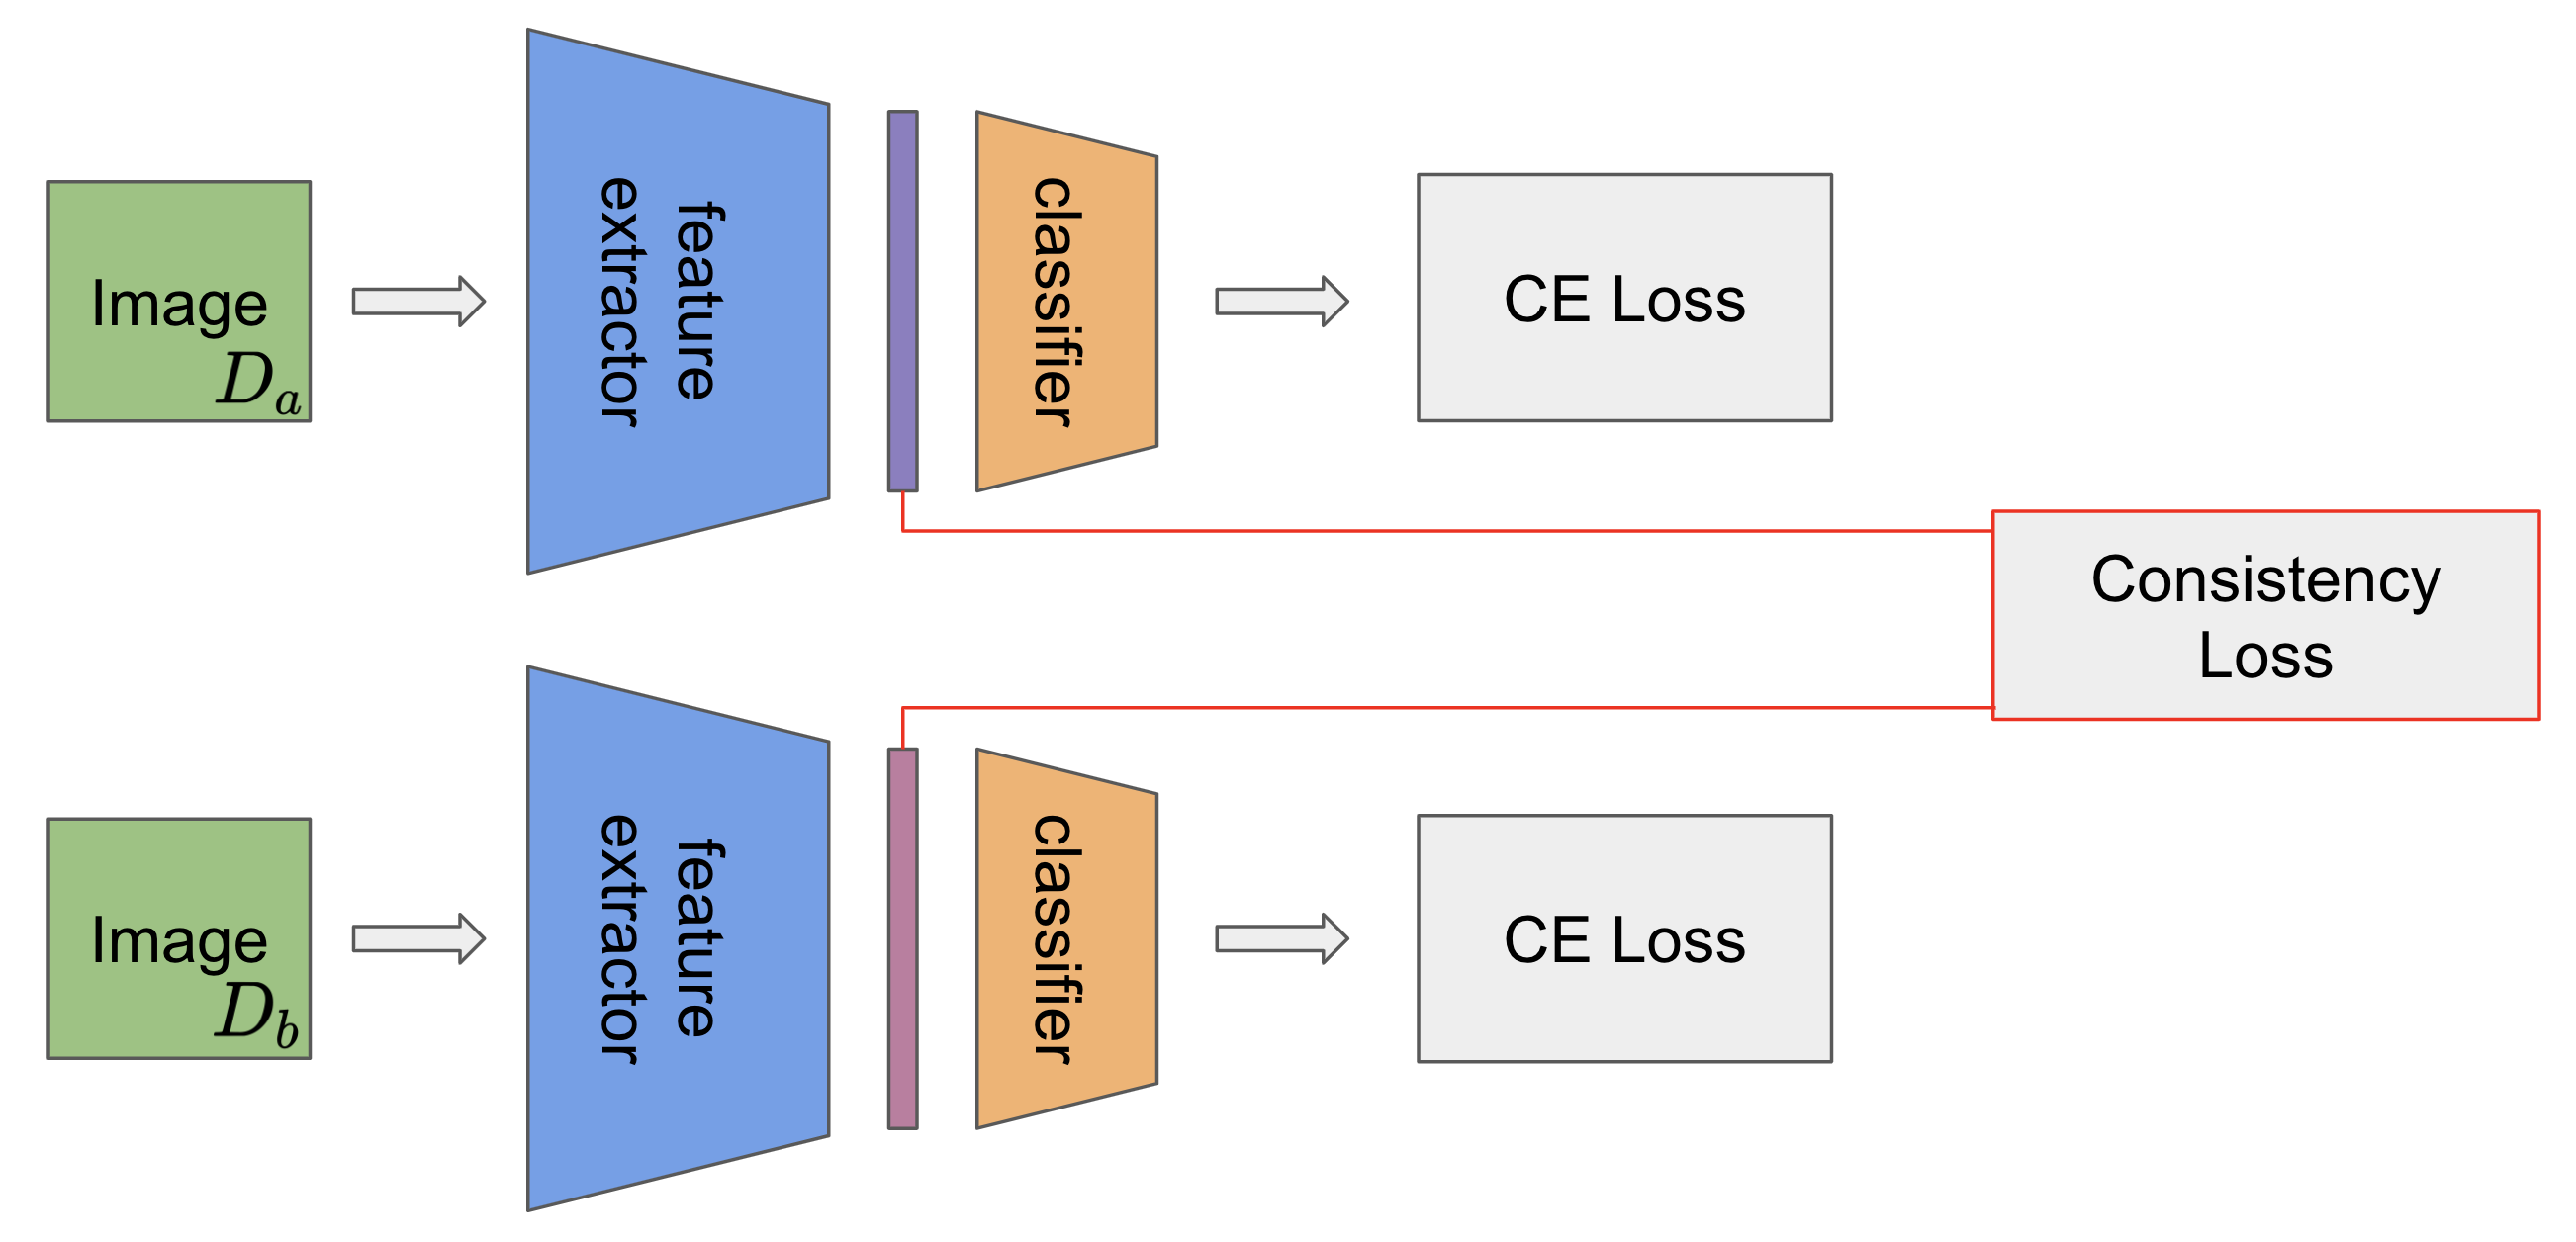
\includegraphics[width=8cm]{figures/model.png}
	\end{tabular}
	\caption{Overview}\label{fig:overview}
\end{figure}

Existing DG studies can be classified into several categories depending on their strategies. Some methods proposed novel model architectures that are robust to domain shift~\cite{Khosla12undobias, Li2017dg}. Others suggested learning algorithms aim to induce a model to fit in a more robust minimum~\cite{li2019episodic, Li2018MLDG, NIPS2018_metareg}. The others adopted losses to learn domain-invariant features by matching feature distributions of the source domains~\cite{Ghifary2015mtae, muandet2013domaingeneralization, mmdaaecvpr2018}. Although these domain-invariant feature learning methods work well, the methods are sub-optimal because they do not utilize task-specific information such as class labels explicitly. 

Our approach also aims to learn domain-invariant features, but the proposed method explicitly adopts the task-specific information. More specifically, we add a simple consistency loss that induces the model to produce similar features when the labels are the same. By using this constraint, the model is expected to learn features that are adequately semantic and constant across domains. Fig.~\ref{fig:overview} shows the overview of the proposed method.

To demonstrate the proposed method works, we conducted experiments on various datasets~\cite{chen2013vlcs, Li2017dg} and models~\cite{He2016resnet}. In the tests, the proposed regularization method consistently improves the performance of the model compared to the baseline method. However, an additional analysis shows that domain-invariant features do not guarantee high performance.

We can summarize our contributions in this works as follows: 1)

